\section{TinyShell测试}

\subsection{测试方法}
针对tsh和参考shell程序tshref,完成测试项目\ref{testbegin}-\ref{testend}的对比测试,并将测试结果截图或者通过重定向保存到文本文件(例如:./sdriver.pl -t trace01.txt -s ./tsh -a "-p" > tshresult01.txt)。

\subsection{测试结果评价}
tsh与tshref的输出在一下两个方面可以不同:

\begin{enumerate}
\item PID
\item 测试文件trace11.txt, trace12.txt和trace13.txt中的/bin/ps命令,每次运行的输出都会不同,但每个mysplit进程的运行状态应该相同。
\end{enumerate}

除了上述两方面允许的差异,tsh与tshref的输出相同则判为正确,如不同则给出原因分析。

\subsection{自测试结果}\label{testcmp}

\subsubsection{测试用例trace01.txt的输出截图(1分)}\label{testbegin}

\begin{figure}[H]
\begin{minipage}[c]{0.5\linewidth}
    \centering
    \caption{tsh测试结果}
    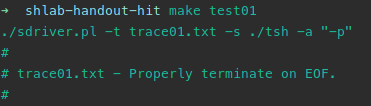
\includegraphics[width=0.7\linewidth]{figures/test01.png}
\end{minipage}
\begin{minipage}[c]{0.5\linewidth}
    \centering
    \caption{tshref测试结果}
    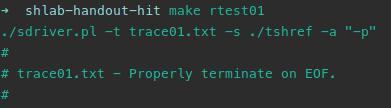
\includegraphics[width=0.7\linewidth]{figures/rtest01.png}
\end{minipage}
\end{figure}

\paragraph{测试结论:}相同

\subsubsection{测试用例trace02.txt的输出截图(1分)}

\begin{figure}[H]
    \begin{minipage}[c]{0.5\linewidth}
        \centering
        \caption{tsh测试结果}
        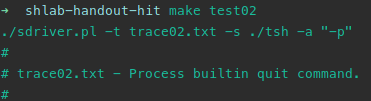
\includegraphics[width=0.7\linewidth]{figures/test02.png}
    \end{minipage}
    \begin{minipage}[c]{0.5\linewidth}
        \centering
        \caption{tshref测试结果}
        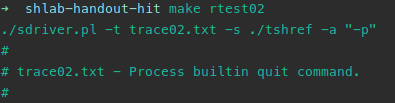
\includegraphics[width=0.7\linewidth]{figures/rtest02.png}
    \end{minipage}
\end{figure}

\paragraph{测试结论:}相同

\subsubsection{测试用例trace03.txt的输出截图(1分)}

\begin{figure}[H]
    \begin{minipage}[c]{0.5\linewidth}
        \centering
        \caption{tsh测试结果}
        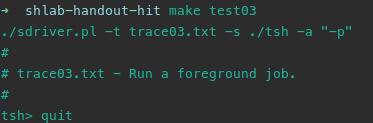
\includegraphics[width=0.7\linewidth]{figures/test03.png}
    \end{minipage}
    \begin{minipage}[c]{0.5\linewidth}
        \centering
        \caption{tshref测试结果}
        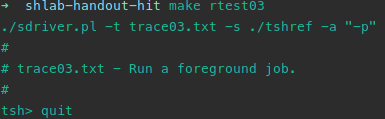
\includegraphics[width=0.7\linewidth]{figures/rtest03.png}
    \end{minipage}
\end{figure}

\paragraph{测试结论:}相同

\subsubsection{测试用例trace04.txt的输出截图(1分)}

\begin{figure}[H]
    \begin{minipage}[c]{0.5\linewidth}
        \centering
        \caption{tsh测试结果}
        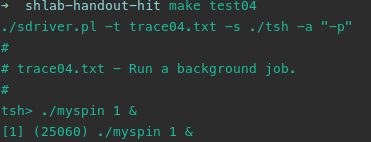
\includegraphics[width=0.7\linewidth]{figures/test04.png}
    \end{minipage}
    \begin{minipage}[c]{0.5\linewidth}
        \centering
        \caption{tshref测试结果}
        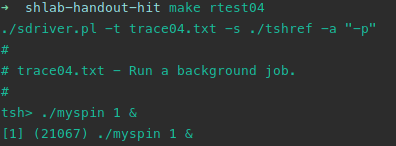
\includegraphics[width=0.7\linewidth]{figures/rtest04.png}
    \end{minipage}
\end{figure}

\paragraph{测试结论:}相同

\subsubsection{测试用例trace05.txt的输出截图(1分)}

\begin{figure}[H]
    \begin{minipage}[c]{0.5\linewidth}
        \centering
        \caption{tsh测试结果}
        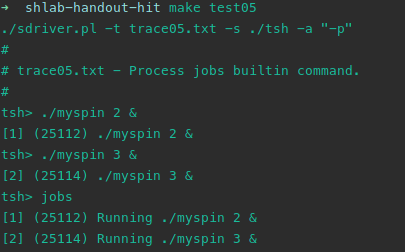
\includegraphics[width=0.7\linewidth]{figures/test05.png}
    \end{minipage}
    \begin{minipage}[c]{0.5\linewidth}
        \centering
        \caption{tshref测试结果}
        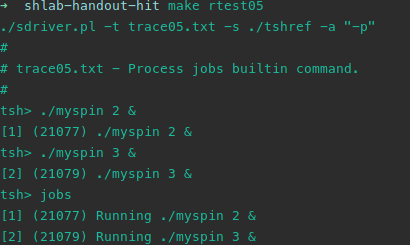
\includegraphics[width=0.7\linewidth]{figures/rtest05.png}
    \end{minipage}
\end{figure}

\paragraph{测试结论:}相同

\subsubsection{测试用例trace06.txt的输出截图(1分)}

\begin{figure}[H]
    \begin{minipage}[c]{0.5\linewidth}
        \centering
        \caption{tsh测试结果}
        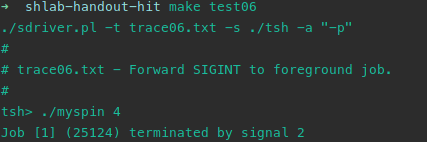
\includegraphics[width=0.7\linewidth]{figures/test06.png}
    \end{minipage}
    \begin{minipage}[c]{0.5\linewidth}
        \centering
        \caption{tshref测试结果}
        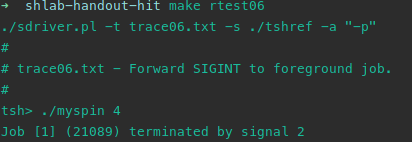
\includegraphics[width=0.7\linewidth]{figures/rtest06.png}
    \end{minipage}
\end{figure}

\paragraph{测试结论:}相同

\subsubsection{测试用例trace07.txt的输出截图(1分)}

\begin{figure}[H]
    \begin{minipage}[c]{0.5\linewidth}
        \centering
        \caption{tsh测试结果}
        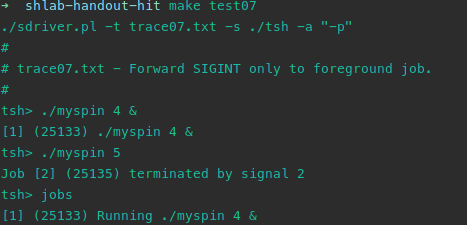
\includegraphics[width=0.7\linewidth]{figures/test07.png}
    \end{minipage}
    \begin{minipage}[c]{0.5\linewidth}
        \centering
        \caption{tshref测试结果}
        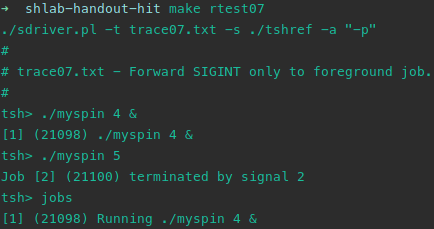
\includegraphics[width=0.7\linewidth]{figures/rtest07.png}
    \end{minipage}
\end{figure}

\paragraph{测试结论:}相同

\subsubsection{测试用例trace08.txt的输出截图(1分)}

\begin{figure}[H]
    \begin{minipage}[c]{0.5\linewidth}
        \centering
        \caption{tsh测试结果}
        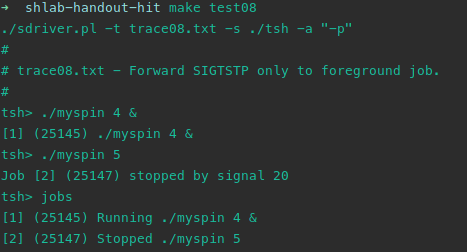
\includegraphics[width=0.7\linewidth]{figures/test08.png}
    \end{minipage}
    \begin{minipage}[c]{0.5\linewidth}
        \centering
        \caption{tshref测试结果}
        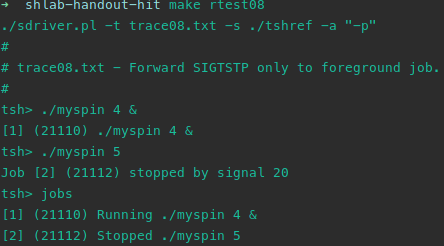
\includegraphics[width=0.7\linewidth]{figures/rtest08.png}
    \end{minipage}
\end{figure}

\paragraph{测试结论:}相同

\subsubsection{测试用例trace09.txt的输出截图(1分)}

\begin{figure}[H]
    \begin{minipage}[c]{0.5\linewidth}
        \centering
        \caption{tsh测试结果}
        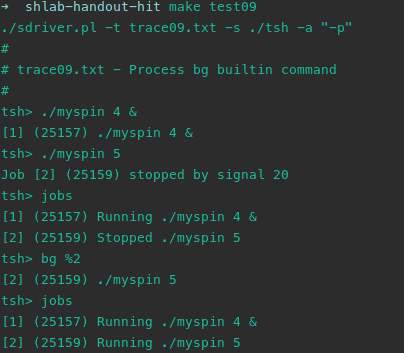
\includegraphics[width=0.7\linewidth]{figures/test09.png}
    \end{minipage}
    \begin{minipage}[c]{0.5\linewidth}
        \centering
        \caption{tshref测试结果}
        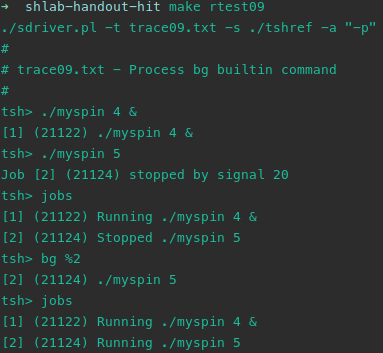
\includegraphics[width=0.65\linewidth]{figures/rtest09.png}
    \end{minipage}
\end{figure}

\paragraph{测试结论:}相同

\subsubsection{测试用例trace10.txt的输出截图(1分)}

\begin{figure}[H]
    \begin{minipage}[c]{0.5\linewidth}
        \centering
        \caption{tsh测试结果}
        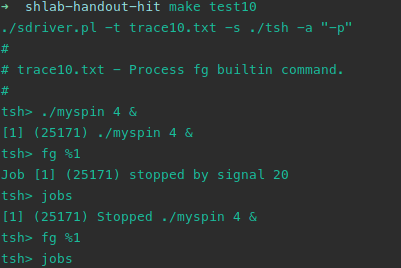
\includegraphics[width=0.7\linewidth]{figures/test10.png}
    \end{minipage}
    \begin{minipage}[c]{0.5\linewidth}
        \centering
        \caption{tshref测试结果}
        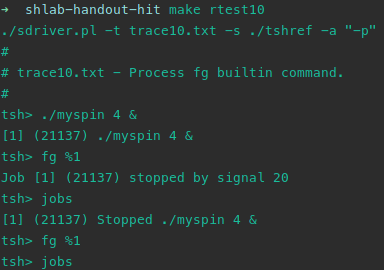
\includegraphics[width=0.65\linewidth]{figures/rtest10.png}
    \end{minipage}
\end{figure}

\paragraph{测试结论:}相同

\subsubsection{测试用例trace11.txt的输出截图(1分)}

\begin{figure}[H]
    \begin{minipage}[c]{0.5\linewidth}
        \centering
        \caption{tsh测试结果}
        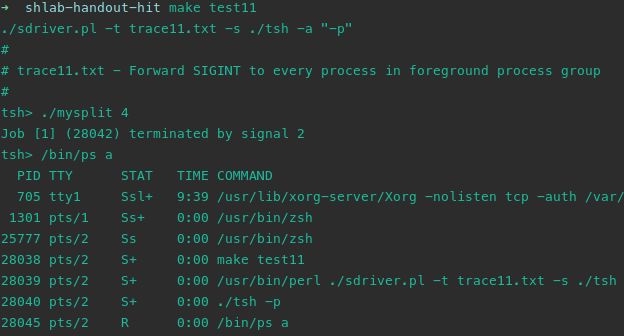
\includegraphics[width=0.99\linewidth]{figures/test11.png}
    \end{minipage}
    \begin{minipage}[c]{0.5\linewidth}
        \centering
        \caption{tshref测试结果}
        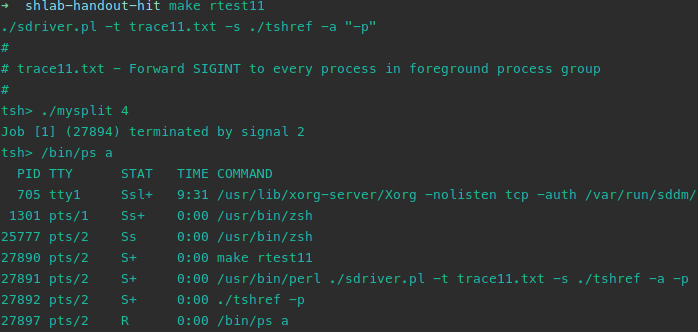
\includegraphics[width=0.99\linewidth]{figures/rtest11.png}
    \end{minipage}
\end{figure}

\paragraph{测试结论:}相同

\subsubsection{测试用例trace12.txt的输出截图(1分)}

\begin{figure}[H]
    \begin{minipage}[c]{0.5\linewidth}
        \centering
        \caption{tsh测试结果}
        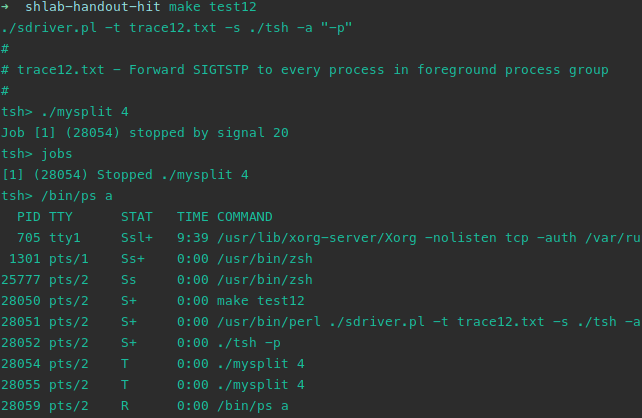
\includegraphics[width=0.99\linewidth]{figures/test12.png}
    \end{minipage}
    \begin{minipage}[c]{0.5\linewidth}
        \centering
        \caption{tshref测试结果}
        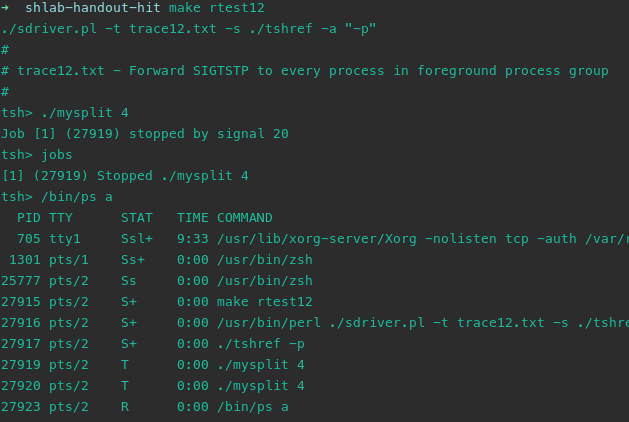
\includegraphics[width=0.99\linewidth]{figures/rtest12.png}
    \end{minipage}
\end{figure}

\paragraph{测试结论:}相同

\subsubsection{测试用例trace13.txt的输出截图(1分)}

\begin{figure}[H]
    \begin{minipage}[c]{0.5\linewidth}
        \centering
        \caption{tsh测试结果}
        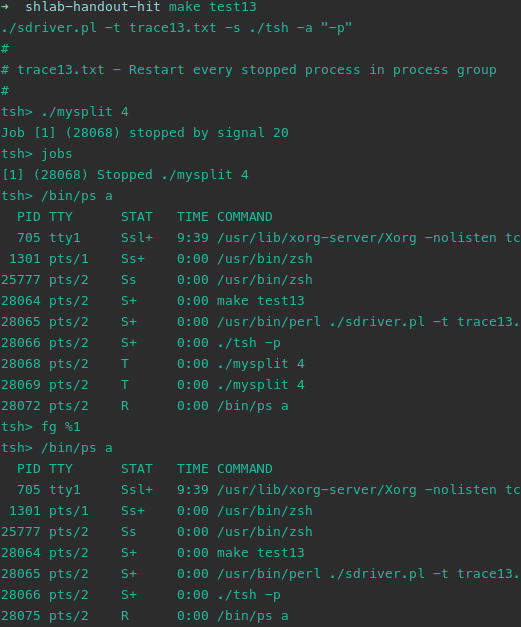
\includegraphics[width=0.9\linewidth]{figures/test13.png}
    \end{minipage}
    \begin{minipage}[c]{0.5\linewidth}
        \centering
        \caption{tshref测试结果}
        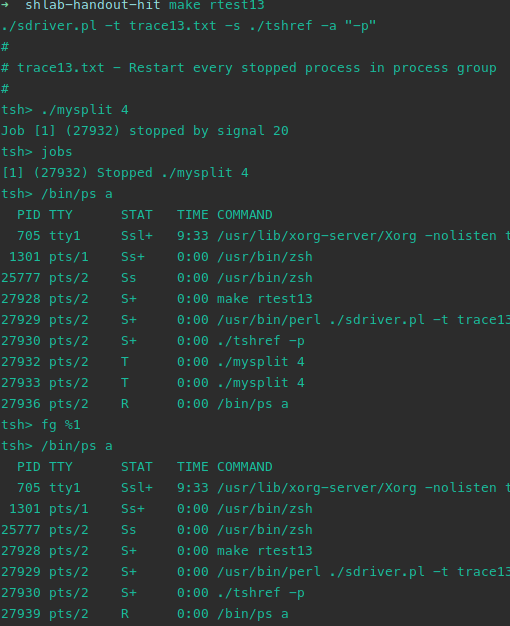
\includegraphics[width=0.9\linewidth]{figures/rtest13.png}
    \end{minipage}
\end{figure}

\paragraph{测试结论:}相同

\subsubsection{测试用例trace14.txt的输出截图(1分)}

\begin{figure}[H]
    \begin{minipage}[c]{0.5\linewidth}
        \centering
        \caption{tsh测试结果}
        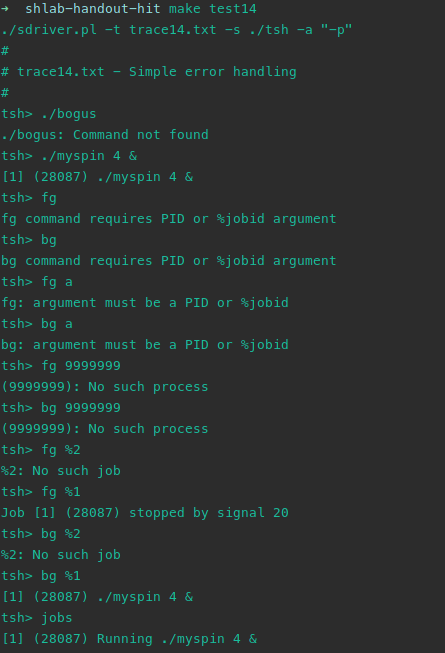
\includegraphics[width=0.7\linewidth]{figures/test14.png}
    \end{minipage}
    \begin{minipage}[c]{0.5\linewidth}
        \centering
        \caption{tshref测试结果}
        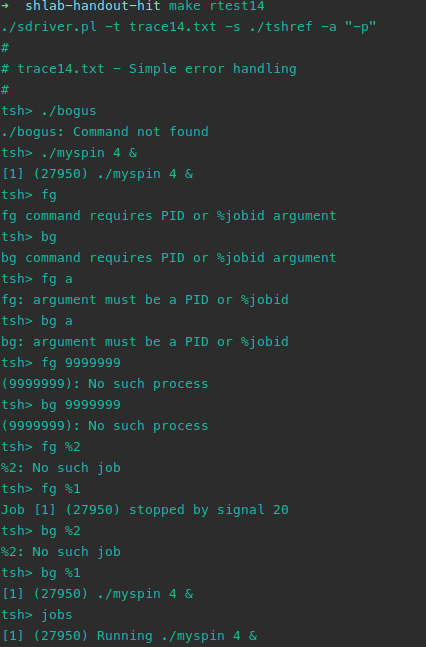
\includegraphics[width=0.7\linewidth]{figures/rtest14.png}
    \end{minipage}
\end{figure}

\paragraph{测试结论:}相同

\subsubsection{测试用例trace15.txt的输出截图(1分)}\label{testend}

\begin{figure}[H]
    \begin{minipage}[c]{0.5\linewidth}
        \centering
        \caption{tsh测试结果}
        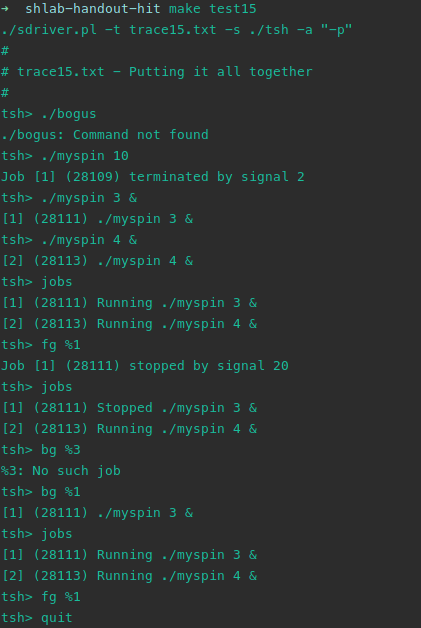
\includegraphics[width=0.7\linewidth]{figures/test15.png}
    \end{minipage}
    \begin{minipage}[c]{0.5\linewidth}
        \centering
        \caption{tshref测试结果}
        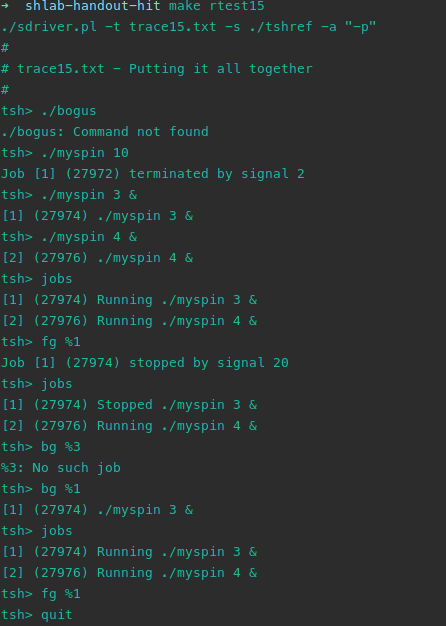
\includegraphics[width=0.7\linewidth]{figures/rtest15.png}
    \end{minipage}
\end{figure}

\paragraph{测试结论:}相同

\subsubsection{测试用例trace16.txt的输出截图(1分)}\label{testend}

\begin{figure}[H]
    \begin{minipage}[c]{0.5\linewidth}
        \centering
        \caption{tsh测试结果}
        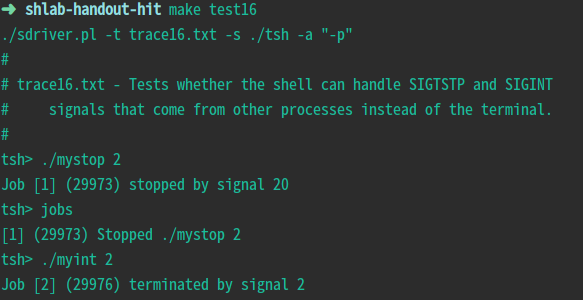
\includegraphics[width=0.7\linewidth]{figures/test16.png}
    \end{minipage}
    \begin{minipage}[c]{0.5\linewidth}
        \centering
        \caption{tshref测试结果}
        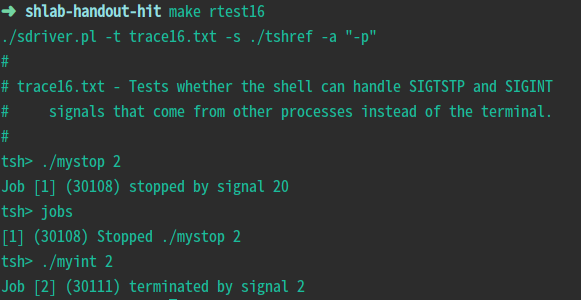
\includegraphics[width=0.7\linewidth]{figures/rtest16.png}
    \end{minipage}
\end{figure}

\paragraph{测试结论:}相同

\subsection{自测试评分}

根据节\ref{testcmp}的自测试结果,程序的测试评分为:\dlmu[3cm]{15}